\documentclass[aspectratio=169]{beamer}

\usepackage[utf8]{inputenc}
\usepackage{lmodern}
\usepackage{pgfplots} \pgfplotsset{compat=1.10} % also includes tikz
% \usetikzlibrary{external} % To speed up compile
% \tikzexternalize[prefix=build/figures/]
% \usepackage{svg} % automatically convert svg and include

\usetheme{Goettingen} % To show sidebar navigation
\setbeamercolor{paleBlue}{fg=black,bg=blue!10!white}

\colorlet{paleBlue}{blue!10!white}
\colorlet{halfBlue}{blue!50!white}
 
%%%%%%%%% helpers
\newcommand{\abs}[1]{\left|#1\right|} % Absolute value
\newcommand{\norm}[1]{\left\|#1\right\|} % Norm
\newcommand{\bC}{\mathbb{C}} % Complex numbers
\newcommand{\bN}{\mathbb{N}} % Natural numbers
\newcommand{\bR}{\mathbb{R}} % Real numbers
\renewcommand{\aa}{\mathbf{a}}
\newcommand{\bb}{\mathbf{b}}
\newcommand{\cc}{\mathbf{c}}
\newcommand{\ee}{\mathbf{e}}
\newcommand{\ff}{\mathbf{f}}
\renewcommand{\gg}{\mathbf{g}}
\newcommand{\hh}{\mathbf{h}}
\newcommand{\nn}{\mathbf{n}}
\newcommand{\rr}{\mathbf{r}}
\newcommand{\uu}{\mathbf{u}}
\newcommand{\vv}{\mathbf{v}}
\newcommand{\ww}{\mathbf{w}}
\newcommand{\xx}{\mathbf{x}}
\newcommand{\yy}{\mathbf{y}}
\newcommand{\zz}{\mathbf{z}}
\newcommand{\aalpha}{\boldsymbol{\alpha}}
\newcommand{\bbeta}{\boldsymbol{\beta}}
\newenvironment{shaded}{\begin{beamercolorbox}[sep=.1em,rounded=true]{paleBlue}}{\end{beamercolorbox}}

%\newcommand{\cover}[1]{\only<1>{\phantom{#1}}\only<2>{#1}}
\newcommand{\cover}[1]{{#1}}



%%%%%%%%%

\title{MA2 -- Part 6 -- Surface integrals}
\subtitle{Weeks 11--12 of MA2 -- Draft lecture slides}
\author[]{Oliver Butterley}
\institute{University of Rome Tor Vergata}
\date{2020/21}
\setbeamercovered{transparent} 

\begin{document}

\frame{\titlepage}

\begin{frame}
    \frametitle{Outline}
    \tableofcontents
\end{frame}


\section{Parametric representation of a surface}

\begin{frame}
    \frametitle{Example: Parametric representation of a hemisphere}


    \structure{Recall:}
    Half circle \(C=\{(x,y): x^2 + y^2=1, y\geq 1\}\) can be parametrized
    \begin{itemize}
        \item \(\aalpha(x):= (x,\sqrt{1-x^2})\), \(x\in [-1,1]\), or
        \item \(\aalpha(t):= (\cos t, \sin t)\), \(t\in [0,\pi]\).
    \end{itemize}

    \vspace{2em}

    \begin{example}[hemisphere]
        The hemisphere \(S = \{(x,y,z): x^2+y^2+z^2=1, z\geq 0\}\) can be parametrized
        \begin{itemize}
            \item \(\rr(x,y):=(x,y,\cover{\sqrt{1-x^2 -y^2}})\), \((x,y)\in\{x^2+y^2 \leq 1\}\), or
            \item \(\rr(u,v):=({\cos u \cos v}, {\sin u \cos v}, \cover{\sin v})\), \((u,v)\in  [0,2\pi] \times [0,\pi/2]\).
        \end{itemize}
    \end{example}

    \begin{block}{Remark}
        Second form can be deduced from spherical coordinates (fixed distance from origin).
    \end{block}


\end{frame}

\begin{frame}
    \frametitle{Example: Parametric representation of a cone}


    \begin{example}[cone]
        The cone \(S = \{(x,y,z): z^2 = x^2+y^2, z\in [0,1]\}\) can be parametrized
        \begin{itemize}
            \item \(\rr(x,y):=(x,y,\cover{\sqrt{x^2+y^2}})\), \((x,y)\in\{x^2+y^2 \leq 1\}\), or
            \item \(\rr(u,v):=(v \cos u, v \sin u, \cover{v})\), \((u,v)\in  [0,2\pi] \times [0,1]\).
        \end{itemize}
    \end{example}


    \begin{block}{Remark}
        Second form can be deduced from spherical coordinates (fixed angle from \(z\)-axis).
    \end{block}

\end{frame}

\section{Fundamental vector product}

\begin{frame}
    \frametitle{Fundamental vector product}

    Consider the parametric surface, denoted \(\rr(T)\),
    \[
        \rr(u,v) := \left(X(u,v),Y(u,v),Z(u,v)\right),
        \quad (u,v)\in T.
    \]

    \begin{definition}[fundamental vector product]
        The vector-valued function
        \[
            \frac{\partial \rr}{\partial u} \times \frac{\partial \rr}{\partial v}
            = \left(\begin{smallmatrix}
                    \partial_{u} X \\ \partial_{u} Y \\ \partial_{u} Z
                \end{smallmatrix}\right)
            \times
            \left(\begin{smallmatrix}
                    \partial_{v} X \\ \partial_{v} Y \\ \partial_{v} Z
                \end{smallmatrix}\right)
        \]
        is called the \emph{fundamental vector product} of the representation \(\rr\).
    \end{definition}

    \begin{block}{Remarks}
        \begin{itemize}
            \item The vector-valued functions \(\frac{\partial \rr}{\partial u}\) and \(\frac{\partial \rr}{\partial v}\) are tangent to the surface,
            \item The fundamental vector product \(\frac{\partial \rr}{\partial u} \times \frac{\partial \rr}{\partial v}\) is normal to the surface,
            \item Represents local scaling of area (small parallelograms).
        \end{itemize}
    \end{block}

\end{frame}

\begin{frame}
    \frametitle{Further details on parametric surface representations}

    \begin{definition}[regular point]
        If \((u,v)\) is a point in \(T\) at which \(\frac{\partial \rr}{\partial u}\) and \(\frac{\partial \rr}{\partial v}\) are continuous and the fundamental vector product is non-zero then \(\rr(u,v)\) is said to be a \emph{regular point} for that representation.
    \end{definition}

    \begin{definition}
        A surface \(\rr(T)\) is said to be smooth if all its points are regular points.
    \end{definition}



\end{frame}


\begin{frame}
    \frametitle{Parametric representation of surface with explicit form}

    Suppose that a surface \(S\) has the form \(z = f(x,y)\), i.e., it is described explicitly.
    \begin{itemize}
        \item We can use \(x,y\) as the parameters and show
              \[
                  \rr(x,y):= \left(x,y,f(x,y)\right),
              \]
        \item The region \(T\) is called the projection of \(S\) onto the \(xy\)-plane,
        \item We compute
              \[
                  \frac{\partial \rr}{\partial x} = \left(\begin{smallmatrix}
                          {1} \\ 0 \\ \partial_{x} f
                      \end{smallmatrix}\right),
                  \quad
                  \frac{\partial \rr}{\partial y} = \left(\begin{smallmatrix}
                          \cover{0} \\ \cover{1} \\ \cover{\partial_{y} f}
                      \end{smallmatrix}\right),
              \]
        \item Consequently
              \[
                  \frac{\partial \rr}{\partial x} \times \frac{\partial \rr}{\partial y}
                  = \left(\begin{smallmatrix}
                          1 \\ 0 \\ \partial_{x} f
                      \end{smallmatrix}\right)
                  \times
                  \left(\begin{smallmatrix}
                          \cover{0} \\ \cover{1} \\ \cover{\partial_{y} f}
                      \end{smallmatrix}\right)
                  =
                  \left(\begin{smallmatrix}
                          \cover{-\partial_{x} f} \\ \cover{-\partial_{y} f} \\ \cover{1}
                      \end{smallmatrix}\right).
              \]

    \end{itemize}


\end{frame}


\begin{frame}
    \frametitle{Example: Hemisphere representation 1}


    \begin{itemize}
        \item     Let \( T:=\{x^2+y^2 \leq 1\}\),
        \item Let
              \(\rr(x,y):=(x,y,\sqrt{1-x^2 -y^2})\).
        \item The surface \(\rr(T)\) is the unit hemisphere.
        \item The fundamental vector product of this representation is
              \[
                  \frac{\partial \rr}{\partial x} \times \frac{\partial \rr}{\partial y}(x,y)
                  =
                  \left(\begin{smallmatrix}
                          \cover{x (1-x^2-y^2)^{-1/2}} \\ \cover{y (1-x^2-y^2)^{-1/2}}  \\ \cover{ 1}
                      \end{smallmatrix}\right)
                  = \cover{z^{-1}} \ \rr(x,y).
              \]
        \item All points are regular except the equator.
    \end{itemize}

\end{frame}


\begin{frame}
    \frametitle{Example: Hemisphere representation 2}


    \begin{itemize}
        \item     Let \( T:= [0,2\pi]\times [0,\pi/2]\),
        \item Let     \(\rr(u,v):= (\cos u \cos v, \sin u \cos v, \sin v)\).
        \item The surface \(\rr(T)\) is the unit hemisphere.
        \item
              \[
                  \frac{\partial \rr}{\partial u}(u,v) = \left(\begin{smallmatrix}
                          -\sin u \cos v \\ \cos u \cos v  \\ 0
                      \end{smallmatrix}\right),
                  \quad
                  \frac{\partial \rr}{\partial v}(u,v) = \left(\begin{smallmatrix}
                          \cover{-\cos u \sin v} \\ \cover{-\sin u \sin v } \\ \cover{\cos v}
                      \end{smallmatrix}\right).
              \]
        \item The fundamental vector product of this representation is
              \[
                  \frac{\partial \rr}{\partial u} \times \frac{\partial \rr}{\partial v}(u,v)
                  = \cover{\cos v }\ \rr(u,v).
              \]
        \item Many points map to the north pole, north pole is not a regular point, many points map to a line between equator and north pole.
    \end{itemize}

\end{frame}

\section{Area of a parametric surface}

\begin{frame}
    \frametitle{Area of a parametric surface}

    \begin{definition}[area of a parametric surface]
        The area of the parametric surface \(S = \rr(T)\) is defined as the double integral
        \[
            \operatorname{Area}(S):= \iint_{T} \norm{\frac{\partial \rr}{\partial u} \times \frac{\partial \rr}{\partial v}} \ dudv.
        \]
    \end{definition}


    \begin{block}{Remarks}
        \begin{itemize}
            \item Similar to the definition of the length of a curve,
            \item We can show that \(\operatorname{Area}(S)\) is \emph{independent} of the choice of representation.
        \end{itemize}
    \end{block}

\end{frame}

\begin{frame}
    \frametitle{Example: Area of a hemisphere}

    \begin{itemize}
        \item     Let, as before, \( T:= [0,2\pi]\times [0,\pi/2]\),
        \item Let    \(\rr(u,v):= (\cos u \cos v, \sin u \cos v, \sin v)\).
        \item    Norm of fundamental vector product:
              \[
                  \norm{\frac{\partial \rr}{\partial x} \times \frac{\partial \rr}{\partial y}(u,v)}
                  = \norm{\cos v \ \rr(u,v)} = \cover{\cos v}.
              \]
        \item
              Hence:     \[
                  \operatorname{Area}(S):= \iint_{T} \cos v \ dudv
                  = \int_{0}^{2\pi} \left[\int_{0}^{\pi/2} \cover{\cos v} \ dv \right] \ du = \cover{2\pi}.
              \]
    \end{itemize}

\end{frame}

\section{Surface integrals}

\begin{frame}
    \frametitle{Surface integrals}

    Similar to line integrals, defined using a parametrization.

    \begin{definition}[surface integral]
        Let \(S = \rr(T)\) be a parametric surface and let \(f\) be a scalar field defined on \(S\).
        The surface integral of \(f\) over \(S\) is defined as
        \[
            \iint_{\rr(T)} f \ dS
            = \iint_{T} f(\rr(u,v))  \norm{\frac{\partial \rr}{\partial u} \times \frac{\partial \rr}{\partial v}(u,v)} \ du dv
        \]
        whenever the double integral on the right exists.
    \end{definition}

    \begin{block}{Remarks:}
        \begin{itemize}
            \item When \(f \equiv 1\) the surface integral reduces to surface area.
            \item If \(f\) is the density of thin material in the form \(S\) then \(\iint_{S} f \ dS\) is the  mass.
            \item We can calculate the centre of mass of material in the form \(S\).
        \end{itemize}

    \end{block}
\end{frame}

\section{Change of parametric representation}

\begin{frame}
    \frametitle{Change of parametric representation}

    \begin{columns}
        \begin{column}{.5\textwidth}
            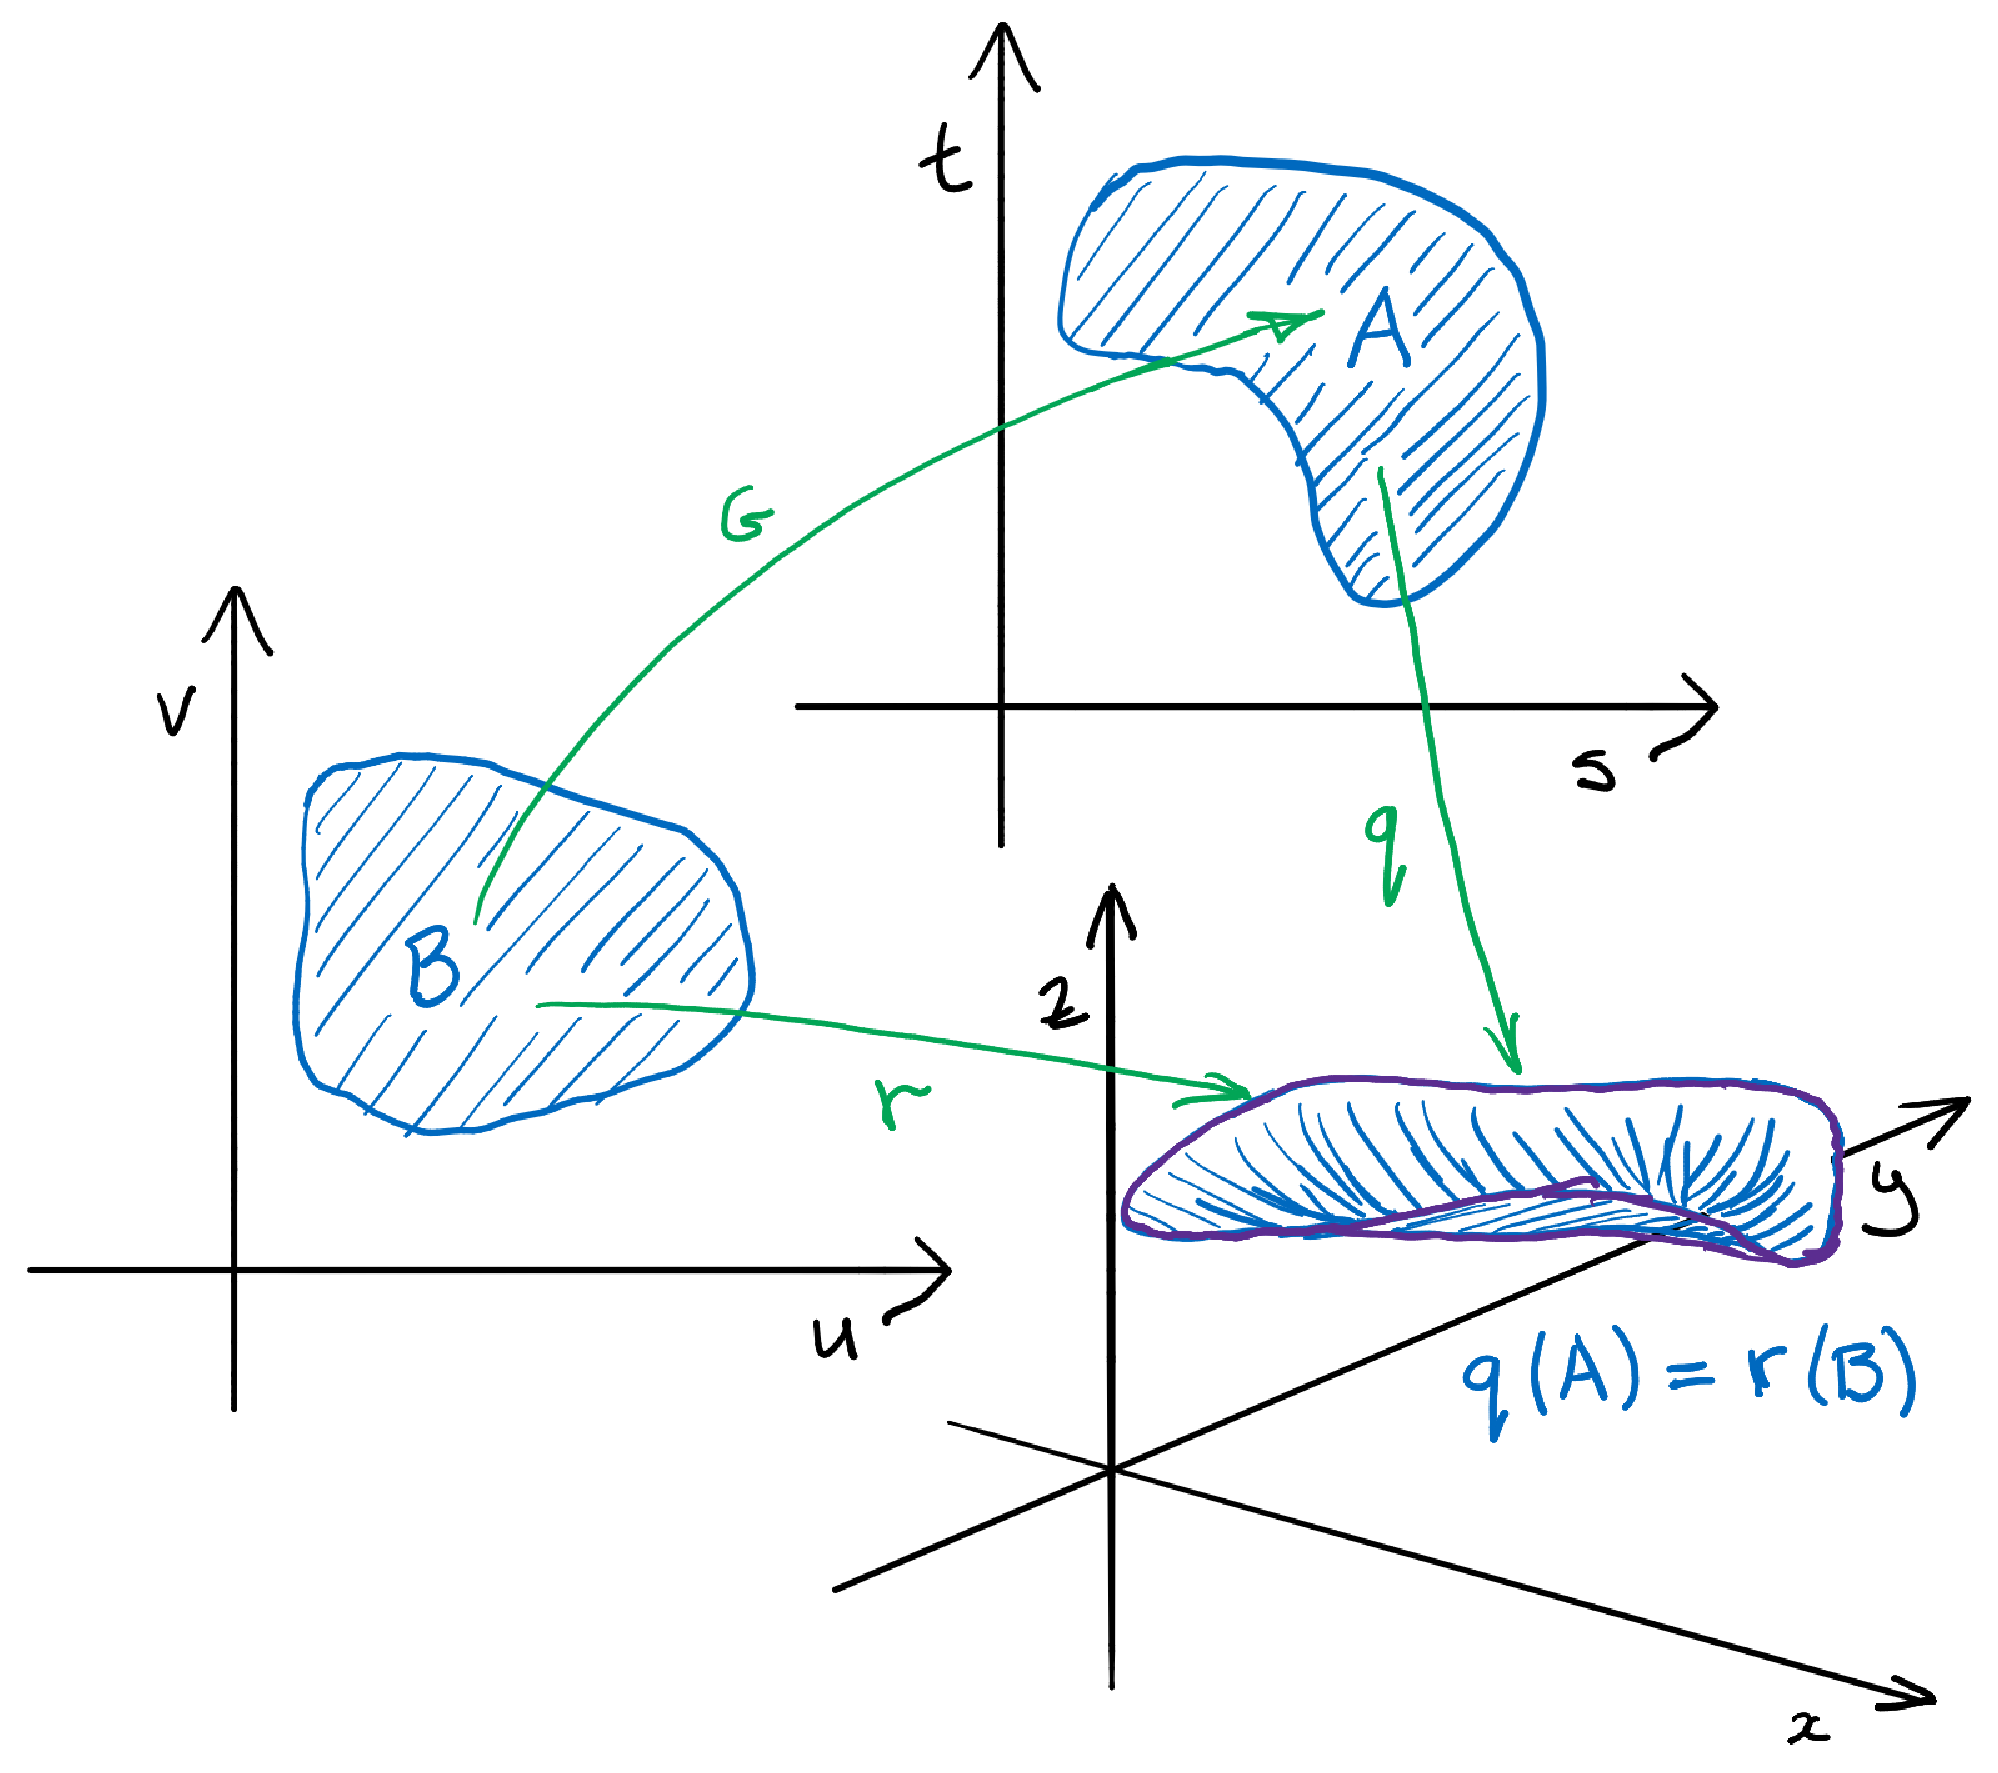
\includegraphics[width=\textwidth]{figures/change-param}
        \end{column}
        \begin{column}{.5\textwidth}
            Suppose that
            \begin{itemize}
                \item \(\mathbf{q}(A)\) and \(\rr(B)\) are both representations of the same surface,
                \item \(\rr = \mathbf{q}\circ G\) for some differentiable \(G:B\to A\).
            \end{itemize}
            Then
            \begin{multline*}
                \iint_{A} f \circ \mathbf{q}  \norm{\frac{\partial  \mathbf{q} }{\partial s} \times \frac{\partial  \mathbf{q} }{\partial t}} \ ds dt \\
                =
                \iint_{B} f \circ \mathbf{r}  \norm{\frac{\partial  \mathbf{r} }{\partial u} \times \frac{\partial  \mathbf{r} }{\partial v}} \ du dv
            \end{multline*}
        \end{column}
    \end{columns}

\end{frame}

\begin{frame}
    \frametitle{Proof of change of parametric representation}

    \begin{enumerate}
        \item Since \(\rr(u,v) = \mathbf{q}(S(u,v),T(u,v))\) we calculate (chain rule and vector product) that
              \[
                  \left[\frac{\partial \rr}{\partial u} \times  \frac{\partial \rr}{\partial v}\right]
                  (u,v)
                  =
                  \left[
                  \left(\frac{\partial \mathbf{q}}{\partial s} \times \frac{\partial \mathbf{q}}{\partial t}\right)
                  \left(\frac{\partial S}{\partial u} \frac{\partial T}{\partial v} -  \frac{\partial S}{\partial v} \frac{\partial T}{\partial u} \right)  \right]
                  (S(u,v),T(u,v)),
              \]
        \item Observe that \(\frac{\partial S}{\partial u} \frac{\partial T}{\partial v} -  \frac{\partial S}{\partial v} \frac{\partial T}{\partial u}\) is the Jacobian determinant associated to change of variables \((u,v) \mapsto  (S(u,v),T(u,v)) \),
        \item Consequently, by the change of variables theorem,
              \begin{multline*}
                  \iint_{A} f \circ \mathbf{q} \ \norm{\frac{\partial  \mathbf{q} }{\partial s} \times \frac{\partial  \mathbf{q} }{\partial t}} \ ds dt
                  =
                  \iint_{B} f \circ \mathbf{r} \  \norm{\frac{\partial  \mathbf{r} }{\partial u} \times \frac{\partial  \mathbf{r} }{\partial v}} \ du dv.
              \end{multline*}
    \end{enumerate}


\end{frame}


\section{Surface integral of a vector field}

\begin{frame}
    \frametitle{Normal vector of a surface}

    \begin{definition}[normal vector]
        Let \(S=\rr(T)\) be a parametric surface
        and let \(\mathbf{N}:= {\frac{\partial  \mathbf{r} }{\partial u} \times \frac{\partial  \mathbf{r} }{\partial v}}\).
        At each regular point there are two unit normals
        \[
            \nn_1 := \frac{\mathbf{N}}{\norm{\mathbf{N}}}
            \quad \text{and} \quad
            \nn_2 := -\nn_1.
        \]
    \end{definition}

    \begin{columns}
        \begin{column}{.5\textwidth}

            \begin{block}{Remark:}
                \begin{itemize}
                    \item If \(\ff\) is a vector field then \(\ff \cdot \nn\) is the component of the flow in direction of \(\nn\).
                \end{itemize}
            \end{block}

        \end{column}
        \begin{column}{.5\textwidth}

        \end{column}
    \end{columns}
\end{frame}

\begin{frame}
    \frametitle{Normal vector and surface integral of a vector field}

    \begin{definition}[surface integral of a vector field]
        Let \(S=\rr(T)\) be a parametric surface and \(\ff\) a vector field.
        The integral
        \[
            \iint_S \ff \cdot \nn \ dS
        \]
        is said to be the \emph{surface integral of \(\ff\) with respect to the normal \(\nn\)}.
    \end{definition}

    \begin{block}{Remarks:}
        \begin{itemize}
            \item \(\iint_S \ff \cdot \nn \ dS
                  = \iint_{T} (\ff\circ \rr) \cdot \nn  \norm{\frac{\partial  \mathbf{r} }{\partial u} \times \frac{\partial  \mathbf{r} }{\partial v}}  \ du dv
                  = \pm \iint_{T} (\ff\circ \rr) \cdot \mathbf{N}    \ du dv\).
            \item \(\iint_S \ff \cdot \nn_1 \ dS = - \iint_S \ff \cdot \nn_2 \ dS\) because \(\nn_1 = - \nn_2\).
        \end{itemize}
    \end{block}

\end{frame}


\section{Curl and divergence}

\begin{frame}
    \frametitle{Curl and divergence}

    \begin{columns}
        \begin{column}{.5\textwidth}
            Suppose that \(\ff = \left(\begin{smallmatrix}
                    f_x \\ f_y \\ f_z
                \end{smallmatrix}\right)\)
            is a vector field.

            \begin{definition}[curl]
                The \emph{curl} of \(\ff\) is defined as
                \[
                    \nabla \times \ff = \begin{pmatrix}
                        \frac{\partial f_z}{\partial y} - \frac{\partial f_y}{\partial z} \\[.5em]
                        \frac{\partial f_x}{\partial z} - \frac{\partial f_z}{\partial x} \\[.5em]
                        \frac{\partial f_y}{\partial x} - \frac{\partial f_x}{\partial y}
                    \end{pmatrix}.
                \]
            \end{definition}

            \begin{definition}[divergence]
                The \emph{divergence} of \(\ff\) is
                \[
                    \nabla \cdot \ff := \frac{\partial f_x}{\partial x} +  \frac{\partial f_y}{\partial y} +  \frac{\partial f_z}{\partial z}.
                \]
            \end{definition}
        \end{column}
        \begin{column}{.5\textwidth}
            \structure{Alternative notation:}
            \begin{itemize}
                \item \(\operatorname{curl} \ff = \nabla \times \ff\)
                \item \(\operatorname{div} \ff = \nabla \cdot \ff\)
            \end{itemize}
            \structure{Properties:}
            \begin{itemize}
                \item If \(\ff = \nabla \varphi\) then \( \nabla \times \ff = \mathbf{0} \),
                \item \(\nabla^2 \varphi := \nabla \cdot (\nabla \varphi) =
                      \frac{\partial^2 \varphi}{\partial x^2} +
                      \frac{\partial^2 \varphi}{\partial y^2} +
                      \frac{\partial^2 \varphi}{\partial z^2}\)
                      is called the Laplacian,
                \item \(\nabla \cdot (\nabla \times \ff) = 0\),
                \item \(\nabla \times (\nabla \times \ff) = \nabla(\nabla\cdot \ff) - \nabla^2 \ff\).
            \end{itemize}

            \begin{theorem}
                Let \(S\subset \bR^3\) be convex. Then \(\nabla \times \ff = \mathbf{0}\) if and only if \(\ff\) is a gradient.
            \end{theorem}
        \end{column}
    \end{columns}

\end{frame}


\begin{frame}
    \frametitle{Examples (curl and divergence)}

    \begin{example}
        If \(\ff(x,y,z) = \begin{pmatrix}
            x \\ y \\ z
        \end{pmatrix}\)
        then
        \(\nabla \times \ff = \mathbf{0}\),
        \(\nabla \cdot \ff = 3\).
    \end{example}

    \begin{example}
        If \(\ff(x,y,z) = \nabla \varphi\)
        then
        \(\nabla \times \ff = \mathbf{0}\).
    \end{example}


    \begin{example}
        If \(\ff(x,y,z) = \begin{pmatrix}
            -y \\ x \\ 0
        \end{pmatrix}\)
        then
        \(\nabla \times \ff = \begin{pmatrix}
            0 \\ 0 \\ 2
        \end{pmatrix}\),
        \(\nabla \cdot \ff = 0\).
    \end{example}

\end{frame}

\section{Theorem of Stokes}

\begin{frame}
    \frametitle{Theorem of Stokes}


    \begin{theorem}[Stokes]
        Let \(S=\rr(T)\) be a parametric surface.
        Suppose that \(T\) is simply connected and that the boundary of \(T\) is mapped to \(C\), the boundary of \(S\).
        Let \(\bbeta\) be a counter clockwise parametrization of the boundary of \(T\) and let \(\aalpha(t) = \rr(\bbeta(t))\).
        Then
        \[
            \iint_{S} (\nabla \times \ff) \cdot \nn \ dS = \int \ff \cdot d\aalpha.
        \]
    \end{theorem}

    \pause

    \begin{proof}[Sketch of proof]
        \begin{enumerate}
            \item Write \(\ff = \left(\begin{smallmatrix}
                      f_x \\ f_y \\ f_z
                  \end{smallmatrix}\right)\)
                  and suppose that \(f_y = f_z = 0\);
            \item Use Green's theorem;
            \item  Conclude for general \(\ff\) by linearity.
        \end{enumerate}
    \end{proof}
\end{frame}


\begin{frame}
    \frametitle{Extension of Stokes' theorem}

    \begin{columns}
        \begin{column}{.5\textwidth}

            Linearity of integrals allows to extend Stokes' theorem to other parametric surfaces:
            \begin{itemize}
                \item Surfaces with holes
                \item Cylinder
                \item Möbius band (does \textbf{not} hold)
                \item Sphere
            \end{itemize}


        \end{column}
        \begin{column}{.5\textwidth}

        \end{column}
    \end{columns}
\end{frame}

\section{Theorem of Gauss}

\begin{frame}
    \frametitle{Theorem of Gauss}

    \begin{theorem}[Gauss]
        Let \(V \subset \bR^3\) be a solid with boundary the parametric surface \(S\) and let \(\nn\) be the outward normal unit vector.
        If \(\ff\) is a vector field then
        \[
            \iiint_{V} \nabla \cdot \ff \ dxdydz = \iint_{S} \ff \cdot \nn \ dS.
        \]
    \end{theorem}


    \begin{proof}[Sketch of proof]

        \begin{enumerate}
            \item Write \(\iiint_V \left(\frac{\partial f_x}{\partial x} + \frac{\partial f_y}{\partial y} + \frac{\partial f_z}{\partial z} \right) \ dx dy dz = \iint_{S} \left(f_x n_x + f_y n_y + f_z n_z\right) \ dS\),
            \item Suffices to show that \(\iiint_V \left(\frac{\partial f_x}{\partial x}  \right) \ dx dy dz = \iint_{S} \left(f_x n_x \right) \ dS\),
            \item Suppose solid is \(xy\)-projectable,
            \item Basic calculus to express \(f_x\) as the integral of the derivative.
        \end{enumerate}
    \end{proof}

    \structure{Remark:}
    Also called the ``Divergence Theorem''.


\end{frame}



\begin{frame}
    \frametitle{Interpretation of divergence as a limit}

    \begin{theorem}
        Let \(V_t\) be the ball of radius \(t>0\) centred at \(\aa\in\bR^3\)
        and let \(S_t\) be its boundary with outgoing unit normal vector \(\nn\).
        Then
        \[
            \nabla\cdot \ff = \lim_{t\to 0} \frac{1}{\operatorname{Vol}(V_t)} \iint_{S_t} \ff \cdot \nn \ dS.
        \]
    \end{theorem}

    \begin{proof}
        Using Gauss' theorem.
    \end{proof}

    \vspace{1em}

    \structure{Remark:}

    Curl can also be written as a similar limit.

\end{frame}


\begin{frame}
    \frametitle{Relation of curl and divergence to the Jacobian matrix}


    \begin{columns}
        \begin{column}{.3\textwidth}

            \[
                \operatorname{Jac}(\ff) =
                \begin{pmatrix}
                    \frac{\partial f_x}{\partial x}
                     & \frac{\partial f_x}{\partial y}
                     & \frac{\partial f_x}{\partial z} \\[1em]
                    \frac{\partial f_y}{\partial x}
                     & \frac{\partial f_y}{\partial y}
                     & \frac{\partial f_y}{\partial z} \\[1em]
                    \frac{\partial f_z}{\partial x}
                     & \frac{\partial f_z}{\partial y}
                     & \frac{\partial f_z}{\partial z}
                \end{pmatrix}
            \]



        \end{column}
        \begin{column}{.6\textwidth}
            \begin{itemize}
                \item     The divergence is the trace of the Jacobian matrix
                \item Every real matrix \(A\) can be written as the sum of a symmetric matrix \(\frac{1}{2}(A + A^{T})\) and a skew-symmetric matrix \(\frac{1}{2}(A - A^{T})\).

            \end{itemize}

        \end{column}
    \end{columns}

    \vspace{2em}

    \[
        \tfrac{1}{2}(\operatorname{Jac}(\ff) - \operatorname{Jac}(\ff)^{T}) =
        \begin{pmatrix}
            0
             & \frac{\partial f_x}{\partial y} - \frac{\partial f_y}{\partial x}
             & \frac{\partial f_x}{\partial z} - \frac{\partial f_z}{\partial x}
            \\[1em]
            \frac{\partial f_y}{\partial x} - \frac{\partial f_x}{\partial y}
             & 0
             & \frac{\partial f_y}{\partial z} - \frac{\partial f_z}{\partial y}
            \\[1em]
            \frac{\partial f_z}{\partial x}  - \frac{\partial f_x}{\partial z}
             & \frac{\partial f_z}{\partial y}  - \frac{\partial f_y}{\partial z}
             & 0
        \end{pmatrix}
    \]


\end{frame}


\end{document}

